\documentclass{article}
\usepackage[a4paper,margin=1in]{geometry}
\usepackage{graphicx}
\usepackage{amsmath}
\usepackage{hyperref}
\hypersetup{colorlinks,urlcolor=blue}
\allowdisplaybreaks

\newcommand{\uvec}[1]{\hat{\textbf{#1}}}

\begin{document}

\section*{Risalita di bolle in un liquido\\{\large Autore: Luca Zoppetti}\\{\large Data: 21 ottobre 2023}}

Si considera una bolla ferma posta sul fondo di una bottiglia. In prima approssimazione, le forze agenti sulla bolla sono la forza di gravità, la forza di Stokes dovuta alla viscosità del liquido e la spinta di Archimede. La somma vettoriale di queste tre forze dà la forza totale esercitata sulla bolla e di conseguenza la sua accelerazione. Per semplicità si studia il caso in cui le bolle si muovono solo verticalmente.

\begin{align}\label{dv}
    m\vec{a} &= \vec{F}_g + \vec{F}_s + \vec{F}_a\notag\\
    ma\uvec{k} &= -mg\uvec{k} - 6\pi\mu r v \uvec{k} + \rho_l g V \uvec{k}\notag\\
    \frac{dv}{dt} &= -g - \frac{6\pi\mu r v}{m} + \frac{\rho_l g V}{m}
\end{align}

\noindent Dove $g$ è l'accelerazione di gravità, $\mu$ è la viscosità del liquido, $r$ il raggio della bolla, $v$ la velocità della bolla, $m$ la massa della bolla, $\rho_l$ la densità del liquido e $V$ il volume della bolla.

La densità della bolla $\rho_b$ può essere espressa come il rapporto $\frac{m}{V}$. Utilizzando la seguente relazione

\begin{equation*}
    m = \rho_b V = \rho_b \frac{4}{3} \pi r^3
\end{equation*}

\noindent si può riscrivere la \eqref{dv} nel modo seguente:

\begin{align}\label{eq2}
    \frac{dv}{dt} &= g - \frac{6 \pi \mu r v}{\rho_b \frac{4}{3}\pi r^3} + \frac{\rho_l}{\rho_b}g\notag\\
    &= - \frac{9}{2} \frac{\mu}{r^2 \rho_b}v + g \left( \frac{\rho_l}{\rho_b} - 1 \right)\notag\\
    &= -\frac{v}{\tau} + g\eta
\end{align}

\noindent dove sono stati posti $\tau = \frac{2}{9} \frac{r^2 \rho_b}{\mu}$, che ha le dimensioni di un tempo, e $\eta = \frac{\rho_l}{\rho_b} - 1$, costante adimensionale maggiore di $0$ perché $\rho_l > \rho_b$.

La \eqref{eq2} si può integrare per parti come segue.

\begin{align}\label{eq3}
    \frac{1}{g} \frac{dv}{-\dfrac{v}{\tau g} + \eta} &= dt\notag\\
    \frac{1}{g} \int_0^{v(t)}\frac{dv'}{-\dfrac{v'}{\tau g} + \eta} &= \int_0^t dt\notag\\
    -\tau \left[\ln{\left( -\frac{v(t)}{\tau g} + \eta \right) - \ln{\left( \eta \right)}}\right] &= t\notag\\
    \ln{\left( -\frac{v(t)}{\tau g \eta} + 1 \right)} &= - \frac{t}{\tau}\notag\\
    v(t) &= \tau g \eta \left( 1 - e^{-t/\tau} \right)
\end{align}

L'altezza $h(t)$ raggiunta dalla bolla al tempo $t$ si trova integrando nuovamente la \eqref{eq3} in $t$.

\begin{align}
    h(t) &= \tau g \eta \int_0^t \left( 1 - e^{-t'/\tau} \right) dt' =\notag\\
    &= \tau g \eta \left[ t + \tau \left(e ^ {-t/\tau} - 1\right) \right] =\notag\\
    &= \tau^2 g \eta \left(\frac{t}{\tau} + e^{-t/\tau} - 1\right)
\end{align}

Con MATLAB si può studiare l'equazione e trovarne una soluzione numerica. I dati utilizzati sono i seguenti:

\begin{table}[ht!]
\centering
    \begin{tabular}{|c|c|c|}
        \hline
        Nome & Valore & Note \\
        \hline
        $g$ & $9.81 m/s^2$ & Accelerazione di gravità \\
        \hline
        $\rho_b$ & $1.0 kg/m^3$ & Densità della bolla, aria come un gas perfetto \\
        \hline
        $\rho_l$ & $916 kg/m^3$ & Densità della vodka al 40\% di alcool\\
        \hline
        $r$ & $5\times10^{-4}m$ & Stima del raggio di una bolla\\
        \hline
        $\mu$ & $2.5\times10^{-3}Pa s$ & Viscosità della vodka al 37.5\% di alcool\\
        \hline
    \end{tabular}
\end{table}

\noindent La densità e la viscosità della vodka sono state ricavate dalle seguenti fonti:
\begin{itemize}
\item \href{https://bartenderly.com/tips-tricks/alcohol-density-chart}{https://bartenderly.com/tips-tricks/alcohol-density-chart}
\item \href{https://www.researchgate.net/figure/a-Measured-mass-density-and-b-viscosity-of-commercial-beverages-as-a-function-of\_fig4\_229017093}{https://www.researchgate.net/figure/a-Measured-mass-density-and-b-viscosity-of-commercial-beverages-as-a-function-of\_fig4\_229017093}
\end{itemize}

Il grafico dell'equazione è riportato di seguito in Fig. \ref{graph}. È praticamente una retta perché $e^{-t/\tau}$ va a zero molto velocemente. Con MATLAB si ricava che il tempo necessario per raggiungere la quota di $20cm$ è $1.0027s$.

\begin{figure}[ht!]
    \centering
    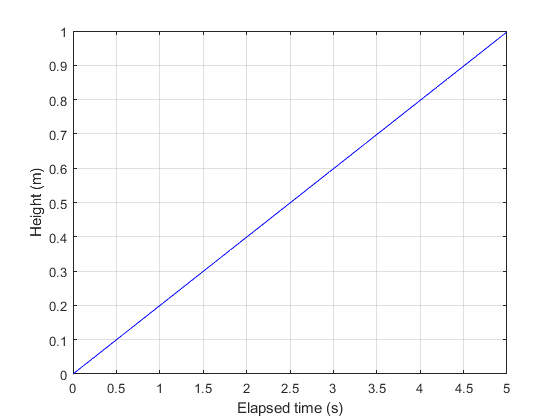
\includegraphics[width=0.8\linewidth]{graph.png}
    \caption{Grafico della funzione $h(t)$. Sull'asse delle ascisse è rappresentato il tempo, sull'asse delle ordinate l'altezza raggiunta.}
    \label{graph}
\end{figure}

\end{document}
